\documentclass[lang=cn,11pt,a4paper]{elegantpaper}
\usepackage[UTF8,scheme=plain]{ctex}
\usepackage[]{booktabs}
\usepackage[]{subfig}
\usepackage[section]{placeins}
\usepackage[]{float}

% 标题信息
\title{一种快速收敛的自适应滑膜控制算法及其在柔性支撑Stewart主动抑振上的应用}
\author{张荣侨}
\institute{清华大学机械工程系}
% \version{1.00}
\date{\today}

\begin{document}

\maketitle

\begin{abstract}
FAST的馈源机构是一个由绳索柔性支撑的Stewart平台,需要对其进行抑振控制。针对动力学模型难以获得的情况,本文提出了一种基于自适应滑膜控制和凸优化的控制方法,
保证了控制对象在给定时间内的收敛特性,同时约束了控制对象的速度、加速度范围,保证控制对象运动过程的稳定和安全。
\keywords{滑膜控制,自适应控制,Stewart 平台}
\end{abstract}

% 引言
\section{引言}

500米口径大型球面射电望远镜(Five hundred meters Aperture Spherical Telescope, FAST项目)是中国自主设计、建造完成的世界上现存最大的,
灵敏度最高的单口径球面射电望远镜,也是国家的九大科技基础设施之一。FAST主体结构修建在贵州独特的喀斯特地貌上,主要包含有主动反射面和馈源支撑系统两个部分,
其中馈源支撑系统上搭载着信号接收装置,需要完成指定的位姿调整才能实现精准的信号接收。馈源支撑系统是一个刚柔耦合二级机构,
由一个6自由度Stewart平台级联在一个6索驱动并联装置上构成\cite{pengFiveHundredMeterApertureSpherical2001}\cite{nanFiveHundredMeter2006}。
在结合力反馈的情况下,FAST位置控制精度可以使得其完成70 MHz到3 GHz的信号观测,而进一步提升馈源支撑系统的位置控制精度可以提升其观测精度,这正是本文的控制目标。

从实验环境的特点来看,由于馈源支撑系统整体悬吊在空中,其所受的外力仅仅只有风扰。根据实地观测结果和对风扰的研究,其外界扰动低频有界。
从实验装置的特点来看,这样的结构成功满足了理论上的运动条件需求,但其自身的动力学特性却带来了其他的控制问题。绳索的弹性特点使得整个馈源舱的系统刚度较低,
很容易受到外界干扰;Stewart平台相对绳索自重不可忽略,其运动过程产生的反作用力会对其自身的运动产生影响,从而使得机构呈现出一定的耦合特性。

针对FAST馈源支撑机构主动抑振问题的研究主要有两个思路,一是进行完整的系统建模,通过模型来完成前馈控制。如刘志华在2015年提出了针对刚柔混联机构的
主动抑振措施,将Ste\\wart平台支链运动也放入模型考虑。在使用绳索弹簧-阻尼模型情况下,将平台的伸缩支链的驱动力视为内力,建立了系统整体的动力学模型,
从而计算得到理论情况伸缩支链运动所需要的动力学耦合补偿项\cite{liuGangRouHunLianJiGouDeZhenDongTeXingJiYiZhenKongZhiYanJiu2015}。
另一个思路则是使用类似自适应控制等的无模型的控制方法。段学超在2010年针对FAST的50m缩尺模型提出了一种自适应交互PID监督控制器。
作者首先通过二阶微分跟踪器在支链长度噪声信号中提取支链速度、加速度信息,然后使用自适应交互算法实时更新PID参数,
实现了Stewart平台的监督控制\cite{duanRouXingZhiChengStewartPingTaiDeFenXiYouHuaYuKongZhiYanJiu2008}。

本文的控制对象属于宏-微系统,对这类系统,其振动特性与刚性的并联机构有所不同,主要区别有两方面:一方面是由于底部的宏观柔性支撑系统自身刚性差,
容易受到外部或者系统内部因素的影响而发生振动;另一方面,柔性支撑系统与其上的刚性并联机构之间存在动力耦合现象,即底部的柔性支撑系统在运动中,
给其基础上的刚性平台带来了科里奥利力等由于非惯性系而出现的力,而上面的刚性平台在运动过程中的反作用力也会对底部支撑系统产生影响,
从而使整个系统的动力学特性变得非常复杂。

对刚柔混联的宏-微系统,学者们主要提出了两种抑振策略:主动抑振策略和被动抑振策略。

被动抑振指的是系统对大的振动不做主动干预,利用系统存在的摩擦力等非保守力和阻尼等因素,使得振动的能量耗散掉,直到振动耗散到可以接受的范围后再进行操作。
主动抑振指的是通过一定的策略,根据观测到的系统状态,对执行器进行连续的控制操作,将目标的振动幅值、频率等控制在可接受的范围。

一般而言,被动抑振适用于精度不太高的情形,研究的学者比较少。对主动抑振策略,有直接通过研究补偿量的方法。从优化角度来看,Yoshikawa使用补偿量最小的原则,
在多自由度的微机器人上进行控制,使基座产生的弹性变形得到补偿,完成了系统的轨迹规划控制\cite{yoshikawaQuasistaticTrajectoryTracking1993}。
从模型角度来看,Parsa利用计算力矩法,对冗余自由度的柔性支撑机器人进行了动力学分析,利用广义逆矩阵方法,使上部刚性机器人产生的振动直接抵消柔性支撑的振动,
并在一个平面的柔性支撑机构上进行了算法验证\cite{parsaControlMacroMicroManipulators2005}。

另一方面,从能量角度来进行宏-微系统的主动抑振。这一思想主要是使振动能量随着时间不断耗散,从而实现抑振。其思想是继承于被动抑振的,
但其可以主动调节控制器来调控能量耗散的情况。Torres基于一定的假设,简化并建立了系统的动力学模型,提出伪被动能量耗散方法,本质是将机器人的特性逼近于一个阻尼器,
同时调节控制器的增益来实现大的能量耗散\cite{torresVibrationControlDeployment1996}。Vliet和Sharf则从振动模态进行考虑,建立了柔性支撑机器人的振动方程,
通过调节机器人控制器的PD增益,保证整体振动与其柔性支撑基础的主阶振动模态相匹配,通过自身结构振动消耗掉宏观的整体振动能量\cite{vlietFrequencyMatchingAlgorithm1998}。

此外,对这类基座晃动的Stewart平台,也有学者专门进行研究。Cerda在2010年针对部署在船舶上的Stewart平台,
使用比例控制和前馈控制来对支链实现直接的调控\cite{cerdasalzmannAmpelmannDevelopmentAccess2010}。
但注意到Stewart机构的惯量相对船舶是可以忽略不计的,因此其问题的耦合性比较弱。Ono等在2020、2021年针对运动基座的Stewart平台,
建立了完整的动力学模型,然后分别测试了$H_{\infty}$、integral sliding mode control(ISMC)和非线性模型预测控制方法,
验证了这三种方法对运动基座的Stwart平台控制的可靠性\cite{onoDevelopmentEquationsMotion2019}\cite{onoControlSimulationsStewart2020}
\cite{onoNonlinearModelPredictive2021}。

总的来说,针对柔性支撑的Stewart机器人,目前的控制方法主要是两种:使用PID/模糊PID的无模型方法和建立(完整)动力学模型/能量模型后的有模型方法。
针对本文的被控对象,其相对于普通的基座晃动Stewart机器人(如船舶上Stewart平台、手术并联Stewart平台)而言,由于基座是绳索牵引悬浮的,
因此Stewart机器人支链的反作用力也会影响基座的运动,这直接使得建立机构的动力学模型和辨识机构动力学参数变得复杂。此外,本模型需要辨识的参数很多,
如果使用有模型的控制方法,需要大量数据和时间进行参数辨识和分析。因此,本文采用无模型的控制思路来进行控制。

\FloatBarrier

\section{问题介绍}

FAST项目目前能够观测到的信号范围为70 MHz到3 GHz,后期的工程目的是达到8GHz。为了实现更高频率的信号观测,需要提升馈源支撑系统的跟踪精度;为了提高终端系统的精度,需要考虑馈源支撑系统本身的自重等带来的反作用力。因此本文针对柔性支撑的并联机构,建立一个结构略不同于FAST项目馈源支撑系统的模型,从而放大支链反作用力因素,研究在给定外部干扰输入幅值和频率的情况下,通过设计控制器来抑制终端振动。

设计的系统运动学模型如图\ref{fig:kinetic_model}所示。基本的符号约定如下,
$A$代表世界坐标系;$B$代表Stewart\\
平台基座动平台所固结的坐标系,是扰动施加的位置;$C$代表Stewart静平台终端所固结的坐标系,是期望控制保持稳定的位置。此外,每个坐标系的中心均用$O_i$表示,比如$A$坐标系中心使用$O_A$表示。每条支链的长度使用$l_i$表示,$i$的值域为$\left\{ 1,2,3,4,5,6 \right\}$,代表6条支链序号。

\begin{figure}[H]
    \centering
    \includegraphics[width=0.4\textwidth]{./imgs/model_structure.png}
    \caption{运动学模型}
    \label{fig:kinetic_model}
\end{figure}

对于FAST本体,根据当地的气象观测数据,有史以来观测到的最大风力干扰为17 m/s,对馈源支撑系统的输入振动幅值为0.5 m\cite{nanFiveHundredMeter2006}。根据相应的有限元分析,支撑系统的前10阶模态为$ 0.004$ $\sim 0.18 \mathrm{Hz}$(另一机构结果为前18阶主频率为$0.15\sim 0.55\mathrm{Hz}$),表明需要注意到的振动输入频率主要为0.18Hz以下\cite{nanFiveHundredMeter2006}。对应于其50 m缩尺模型,指定的振动输入为幅值40 mm,频率$ 0.02 \sim 0.18 \mathrm{Hz}$,得到的最终闭环幅值控制精度为$ 15\sim 20 \mathrm{mm}$\cite{duanRouXingZhiChengStewartPingTaiDeFenXiYouHuaYuKongZhiYanJiu2008}。结合设计的这两个实验范围,本文装置的输入幅值最大为20 mm,输入频率保持为$ 0.02\sim 0.18 \mathrm{Hz}$。对于精度评价指标,闭环的幅值控制精度对应缩尺到$ 7.5\sim 10 \mathrm{mm}$。

% 可以发现,待控制的柔性支撑的Stewart平台,其具有非线性时变的特征,难以对其进行准确的建模和分析。因此具体来说,需要完成的控制器要满足下面几个特征:

% \begin{enumerate}
%     \item 控制器是基于无模型的控制
%     \item 控制器对噪声鲁棒,抗干扰能力强
%     \item 控制器输出受限,保证仪器安全
%     \item 控制器收敛速度快
% \end{enumerate}
\FloatBarrier


\section{控制算法}

本文基于\cite{plestanNewMethodologiesAdaptive2010}提出了一种新的自适应滑膜控制算法来解决上面提出的问题。系统总的控制框图如下:

\begin{figure}[H]
    \centering
    \includegraphics[width=0.6\textwidth]{./imgs/control_model.png}
    \caption{控制框图}
    \label{fig:control_model}
\end{figure}

如图\ref{fig:control_model}所示,控制器由三部分组成:第一级是运动学逆解,用于根据B平台位姿计算出理论上的6条支链长度;第二级是设计的一个凸优化轨迹规划器,用于限制支链运动的最大速度和加速度,保证机构安全;第三级是提出的自适应滑膜控制器,用于自适应地控制输出的实际轴长,减小误差和支链运动带来的影响;

将控制对象抽象为式子(\ref{eqn:sys_model})描述的微分方程,提出下面的控制算法。

\begin{equation}
    \dot{x}=f\left( x \right) +g\left( x \right) u
    \label{eqn:sys_model}
\end{equation}

其中$x\in R^n$是系统的状态变量,$f(x)$和g$(x)$是在$x$定义域内有界的。假定控制的滑膜变量为$\sigma(x,t)$,目的是使得$\sigma=0$。

根据系统方程(\ref{eqn:sys_model}),有

\begin{equation}
    \begin{array}{c}
        \dot{\sigma}=\frac{\partial \sigma}{\partial x}\dot{x}+\frac{\partial \sigma}{\partial t}\\
        =\underset{\varPsi \left( x,t \right)}{\underbrace{\frac{\partial \sigma}{\partial x}f\left( x \right) +\frac{\partial \sigma}{\partial t}}}+\underset{\varGamma \left( x,t \right)}{\underbrace{\frac{\partial \sigma}{\partial x}g\left( x \right) u}}\\
    \end{array}
\end{equation}

根据假设,系统满足:
\begin{equation}
    \left| \varPsi \right|\le \varPsi _M, 0<\varGamma _m\le \varGamma \le \varGamma _M
    \label{eqn:sys_constrain}
\end{equation}

提出自适应滑膜控制器,满足:

\begin{equation}
    \begin{array}{c}
        u=-K\tanh \left( \sigma \left( x,t \right) \right)\\
        \dot{K}=\begin{cases}
        \bar{K}\left| \sigma \left( x,t \right) \right|\mathrm{sign}\left( \left| \sigma \left( x,t \right) \right|-\varepsilon \right)\\
        \mu\\
    \end{cases}\qquad \begin{array}{c}
        \mathrm{if}\quad K>\mu\\
        \mathrm{if}\quad K\le \mu\\
    \end{array}\\
        \bar{K}=\bar{K}_0\exp \left( C_e\left| \sigma \left( x,t \right) \right| \right) , \varepsilon =T_eK\\
    \end{array}
    \label{eqn:controller}
\end{equation}

其中$K\left( 0 \right) >0,C_e>0,\bar{K}_0>0,T_e >0,\mu >0$且$\mu$很小。那么,可以证明,这样的控制器有下面2个特点。

\begin{lemma}
    K存在上界
    \label{lemma1}
\end{lemma}

\begin{figure}[H]
    \centering
    \includegraphics[width=0.6\textwidth]{imgs/math_proof_1.png}
    \caption{一个调节周期内$\sigma$和$K$的变化曲线}
    \label{fig:math_proof_1}
\end{figure}

假定一开始$K>\mu$,$\left| \sigma \left( x,t \right) \right|>\varepsilon$,那么此时K开始增长,且满足增长速率:

\begin{equation}
    \begin{array}{c}
        \dot{K}=\bar{K}_0\exp \left( C_e\left| \sigma \right| \right), \left| \sigma \right|\ge \underset{K_c>0}{\underbrace{\bar{K}T_e}}K\\
        \Rightarrow K\ge \exp \left( K_ct+c \right)\\
    \end{array}
    \label{eqn:l1_Kinit}
\end{equation}

这表明$K$的数值呈指数上升。从而K会一直增加,直到一个$t_1$时刻,此时$u$足够大使得滑膜变量$\sigma$开始减小,即式子(\ref{eqn:l1_sigma_decrease})所示。

\begin{equation}
    \begin{array}{c}
        \dot{\sigma}=\varPsi \left( x,t \right) +\varGamma \left( x,t \right) u\\
        \left| \varPsi \right|\le \varPsi _M, 0<\varGamma _m<\varGamma <\varGamma _M\\
        \Rightarrow \dot{\sigma}\le \varPsi _M+\varGamma _mu, u<0\\
        \Rightarrow \dot{\sigma}<0\quad \mathrm{if}\quad \left| u \right|>\frac{\varPsi _M}{\varGamma _m}\\
    \end{array}
    \label{eqn:l1_sigma_decrease}
\end{equation}

注意到这里$u$增长是指数形式的,从而这里的$t_1$不会太大,基本上是对数时间达到该点。

在此之后K继续增大,直到$\sigma$再次下降到$\varepsilon$,此时K在$t_2$时刻达到最大。注意到从$t_1$到$t_2$过程中,输出$u$相比从开始到$t_1$的阶段更大,因此对我们的系统(\ref{eqn:sys_model})而言,其滑膜变量减小速度比前一段更快,即表明$\left\| t_2-t_1 \right\| \le \left\| t_1 \right\| $,从而这里的K最大值是有限的。继续这个进程,K开始减小,直到$t_3$时刻,K太小以至于无法抵消外界扰动(也就是使得$\sigma$斜率再次为0)。再进一步此时K保持减小,直到误差增大到初始时刻的情况,达到时刻$t_4$,回到一开始的起点。

由于$t_i$时刻是有限的,因此K增加的范围也是有限的。在上述的整个过程中,$t_2$处取得有限的最大值,这表明K存在上界。

\begin{lemma}
    对上面的非线性系统和控制方法,存在有限的时间$t_F>0$使得实际滑模面在所有$t>t_F$的时候成立,即:
\begin{eqnarray}
    \begin{array}{c}
        \left| \sigma \left( x,t \right) \right|<\delta , \forall t\ge t_F\\
        \delta =\ln \left( \exp \left( \sigma _0 \right) +\frac{1}{2\varGamma _m\bar{K}_0}\left( \frac{\varPsi _M}{T_eK\left( 0 \right)}-\varGamma _mK\left( 0 \right) \right) ^2 \right)\\
        t_F=\frac{2\mathrm{arcsech} \left( \sqrt{\frac{-2a}{{\dot{\sigma}_0}^2-2a\exp \left( \sigma _0 \right)}} \right)}{\sqrt{{\dot{\sigma}_0}^2-2a\exp \left( \sigma _0 \right)}}\\
        \sigma _0=\varepsilon ^+\ge \varepsilon =T_eK\left( 0 \right) ,\dot{\sigma}_0=\varPsi _M-\varGamma _m\varepsilon ^+K\left( 0 \right)\\
        a=-\varGamma _m\bar{K}_0\left( \varepsilon ^+ \right) ^2\\
    \end{array}
    \label{eqn:l2_actual_sliding_model}
\end{eqnarray}
\label{lemma2}
\end{lemma}

考虑李雅普诺夫函数,有:

\begin{eqnarray}
    V=\frac{1}{2}\sigma ^2+\frac{1}{2\gamma}\left( K-K^* \right) ^2
    \label{enq:l2_lyaponiv}
\end{eqnarray}

其中$K^*$是K的上界。对V时间微分有式子(\ref{eqn:l2_dV}):

\begin{eqnarray}
    \begin{array}{c}
        \dot{V}=\sigma \left( \varPsi -\varGamma K\tanh \left( \sigma \right) \right) +\frac{1}{\gamma}\left( K-K^* \right) \bar{K}\left| \sigma \right|\mathrm{sign}\left( \left| \sigma \right|-\varepsilon \right)\\
        \le \varPsi _M\left| \sigma \right|-\varGamma _mK\left| \sigma \right|+\frac{1}{\gamma}\left( K-K^* \right) \bar{K}\left| \sigma \right|\mathrm{sign}\left( \left| \sigma \right|-\varepsilon \right)\\
        =\varPsi _M\left| \sigma \right|-\varGamma _mK\left| \sigma \right|+\underset{\text{构造项}}{\underbrace{\varGamma _mK^*\left| \sigma \right|-\varGamma _mK^*\left| \sigma \right|}}+\frac{1}{\gamma}\left( K-K^* \right) \bar{K}\left| \sigma \right|\mathrm{sign}\left( \left| \sigma \right|-\varepsilon \right)\\
        =\left( \varPsi _M-\varGamma _mK^* \right) \left| \sigma \right|+\left( K-K^* \right) \left( -\varGamma _m\left| \sigma \right|+\frac{1}{\gamma}\bar{K}\left| \sigma \right|\mathrm{sign}\left( \left| \sigma \right|-\varepsilon \right) \right)\\
    \end{array}
    \label{eqn:l2_dV}
\end{eqnarray}

进一步添加构造项$\beta_{K}>0$有:

$$\begin{array}{c}
	\dot{V}\leq \left( \varPsi _M-\varGamma _mK^* \right) \left| \sigma \right|+\left( K-K^* \right) \left( -\varGamma _m\left| \sigma \right|+\frac{1}{\gamma}\bar{K}\left| \sigma \right|\mathrm{sign}\left( \left| \sigma \right|-\varepsilon \right) \right)\\
	+\beta _K\left| K-K^* \right|-\beta _K\left| K-K^* \right|\\
\end{array}$$

根据引理\ref{lemma1},K存在上界,则有式子(\ref{eqn:l2_Kg0})

\begin{equation}
    K\left( t \right) -K^*<0,\forall t>0
    \label{eqn:l2_Kg0}
\end{equation}

从而有式子(\ref{eqn:l2_dVl0})

\begin{equation}
    \begin{array}{c}
        \dot{V}\leq -\underset{\beta _{\sigma}>0}{\underbrace{\left( -\varPsi _M+\varGamma _mK^* \right) }}\left| \sigma \right|-\beta _K\left| K-K^* \right|\\
        -\underset{\xi}{\underbrace{\left| \underset{<0}{\underbrace{K-K^*}} \right|\left( -\varGamma _m\left| \sigma \right|+\frac{1}{\gamma}\bar{K}\left| \sigma \right|\mathrm{sign}\left( \left| \sigma \right|-\varepsilon \right) -\beta _K \right) }}\\
    \end{array}
    \label{eqn:l2_dVl0}
\end{equation}

这意味着式子(\ref{eqn:l2_dVl0_1}):

\begin{equation}
    \begin{array}{c}
        \dot{V}\leq -\beta _{\sigma}\left| \sigma \right|-\beta _K\left| K-K^* \right|-\xi\\
        =-\beta _{\sigma}\sqrt{2}\frac{\left| \sigma \right|}{\sqrt{2}}-\beta _K\sqrt{2\gamma}\frac{\left| K-K^* \right|}{\sqrt{2\gamma}}-\xi\\
        \dot{V} \le -\min \left\{ \beta _{\sigma}\sqrt{2}, \beta _K\sqrt{2\gamma} \right\} \left( \frac{\left| \sigma \right|}{\sqrt{2}}+\frac{\left| K-K^* \right|}{\sqrt{2\gamma}} \right) -\xi\\
        \le -\beta V^{1/2}-\xi, \quad \beta =\min \left\{ \beta _{\sigma}\sqrt{2}, \beta _K\sqrt{2\gamma} \right\}\\
    \end{array}
    \label{eqn:l2_dVl0_1}
\end{equation}

现在分析$\xi$的情况。

\textbf{Case1: $\left| \sigma \right|>\varepsilon$}

由于$\left| \sigma \right|>\varepsilon$,此时有式子(\ref{eqn:l2_xi_1})

\begin{equation}
    \begin{array}{c}
        \xi =-\varGamma _m\left| \sigma \right|+\frac{1}{\gamma}\bar{K}_0\exp \left( \left| \sigma \right| \right) \left| \sigma \right|\mathrm{sign}\left( \left| \sigma \right|-\varepsilon \right) -\beta _K>0\\
        \Longleftrightarrow \gamma <\frac{\bar{K}_0\exp \left( \left| \sigma \right| \right) \left| \sigma \right|}{\varGamma _m\left| \sigma \right|+\beta _K}\\
    \end{array}
    \label{eqn:l2_xi_1}
\end{equation}

注意到右边函数是增函数,因此取:

\begin{equation}
    \gamma <\frac{\bar{K}_0\exp \left( \varepsilon \right) \varepsilon}{\varGamma _m\varepsilon +\beta _K}
\end{equation}

对于给定的$\varepsilon$,存在这样的$\gamma$。
此时有式子(\ref{eqn:l2_dV_c1})

\begin{equation}
    \dot{V}\le -\beta V^{1/2}-\xi \le -\beta V^{1/2}
    \label{eqn:l2_dV_c1}
\end{equation}

根据李雅普诺夫收敛的性质,这表明在任何$\left| \sigma \right|>\varepsilon$的条件下,控制对象在有限时间内收敛。

\textbf{Case2: $\left| \sigma \right|<\varepsilon$}

此时$\xi$可能为负,这意味着李雅普诺夫的思路不能完全成功。但可以注意到,一旦$\left| \sigma \right|>\varepsilon$,立马问题就解决了。因此我们需要考虑的问题从最坏情形来分析,实际上是在考虑下面的情况:

在$\left| \sigma \right|<\varepsilon$切换到$\left| \sigma \right|>\varepsilon$之后,V从Case1情形,即$\left| \sigma \right|>\varepsilon$收敛回$\left| \sigma \right|<\varepsilon$所需要花费的成本。
Case1中使用李雅普诺夫稳定性分析证明了一定是会收敛回来的,而且其耗费的时间是对数的。因此问题化简为考虑最坏情形的误差成本——分析状态切换需要的时间代价和精度问题。

记$\sigma _0=\sigma \left( 0 \right) =\varepsilon ^+>\varepsilon$,$K_0=\mathcal{K} \left( 0 \right) =K\left( 0 \right)$。不失一般性,可以假设$\sigma_0>0$,否则其会一直增长。考虑最坏情形,即式子(\ref{eqn:l2_worst_case}):

\begin{equation}
    \begin{array}{c}
        \dot{\sigma}=\underset{P_m}{\underbrace{\varPsi _M}}-\underset{T_m}{\underbrace{\varGamma _m\varepsilon ^+}}K\\
        \dot{K}=\bar{K}_0\sigma \exp \left( \sigma \right) \ge \underset{K_m}{\underbrace{\bar{K}_0\varepsilon ^+}}\exp \left( \sigma \right)\\
        \sigma \left( 0 \right) =\varepsilon ^+>T_eK\left( 0 \right)\\
    \end{array}
    \label{eqn:l2_worst_case}
\end{equation}

这里的最坏情形意思是放任$\sigma$增大,此时偏离滑模面的误差最大的情况。

注意这里$C_e>0$,对$\sigma$而言,实际上代表着一个时间上的放缩,因此可以假设$C_e=1$。

从而问题可以转化为求解方程(\ref{eqn:l2_dsigma}):

\begin{equation}
    \begin{array}{c}
        \ddot{\sigma}=\underset{a}{\underbrace{-T_mK_m}}\exp \left( \sigma \right)\\
        \sigma \left( 0 \right) =\varepsilon ^+>T_eK\left( 0 \right)\\
    \end{array}
    \label{eqn:l2_dsigma}
\end{equation}

通过令$\sigma(t)=e^{f(t)}$进行变换,可以得到式子(\ref{eqn:l2_dsigma})的解为式子(\ref{eqn:l2_sigma}):

\begin{equation}
    \sigma \left( t \right) =\log \left( \frac{c_1\left( \tanh ^2\left( \frac{1}{2}\sqrt{c_1(c_2+t)^2} \right) -1 \right)}{2a} \right) 
    \label{eqn:l2_sigma}
\end{equation}

其中$c_1,c_2$为待定项,根据$\sigma$的初值条件确定。

带入原问题的初值条件,可以将$\sigma$表示为式子(\ref{eqn:l2_sigma_real}):

\begin{equation}
    \begin{array}{c}
        \sigma \left( t \right) =\ln \left( \frac{-s}{2a}\left( 1+\tan \left( \frac{1}{2}\left( it\sqrt{s}-2i\tanh ^{-1}\left( \frac{\dot{\sigma}_0}{\sqrt{s}} \right) \right) \right) \right) \right)\\
        s={\dot{\sigma}_0}^2-2a\exp \left( \sigma _0 \right) >0, a<0\\
    \end{array}
    \label{eqn:l2_sigma_real}
\end{equation}

考虑其在时间上的最大值,直接微分并求零点得到最大值满足式子(\ref{eqn:l2_sigma_max}):

\begin{equation}
    \begin{array}{c}
        \sigma _{\max}=\ln \left( \exp \left( \sigma _0 \right) -\frac{{\dot{\sigma}_0}^2}{2a} \right) =\ln \left( \exp \left( \sigma _0 \right) +\frac{{\dot{\sigma}_0}^2}{2\varGamma _m\bar{K}_0\left( \varepsilon ^+ \right) ^2} \right)\\
        \sigma _0=\varepsilon ^+, \dot{\sigma}_0=\varPsi _M-\varGamma _m\varepsilon ^+K\left( 0 \right)\\
        t_{\max}=\frac{2\mathrm{arcsech} \left( \sqrt{\frac{-2a}{{\dot{\sigma}_0}^2-2a\exp \left( \sigma _0 \right)}} \right)}{\sqrt{{\dot{\sigma}_0}^2-2a\exp \left( \sigma _0 \right)}}, a=-\varGamma _m\bar{K}_0\left( \varepsilon ^+ \right) ^2\\
    \end{array}
    \label{eqn:l2_sigma_max}
\end{equation}

从幅值收敛情况来看,整体的极限情况偏差距离是有限的,且注意到$\varepsilon ^+\ge \varepsilon =T_eK\left( 0 \right)$,这表明式子(\ref{eqn:l2_sigma_max_1}):

\begin{equation}
    \begin{array}{c}
        \sigma _{\max}=\ln \left( \exp \left( \sigma _0 \right) +\frac{1}{2\varGamma _m\bar{K}_0}\left( \underset{L}{\underbrace{\frac{\varPsi _M}{\varepsilon ^+}-\varGamma _mK\left( 0 \right) }} \right) ^2 \right)\\
        \le \ln \left( \exp \left( \sigma _0 \right) +\frac{1}{2\varGamma _m\bar{K}_0}\left( \frac{\varPsi _M}{T_eK\left( 0 \right)}-\varGamma _mK\left( 0 \right) \right) ^2 \right)\\
        \sigma _0=\varepsilon ^+\ge \varepsilon =T_eK\left( 0 \right) , L=\frac{\dot{\sigma}_0}{\varepsilon ^+}>0\\
    \end{array}
    \label{eqn:l2_sigma_max_1}
\end{equation}

注意到$\dot{\sigma}_0>0$,这使得$L>0$。从而可以发现K越大,收敛前的超差越小。

相比Plestan所提出模型最坏情况下的超差函数,这里的函数是对数的,在大误差的时候收敛情况更优。

Plestan论文中的超差函数\cite{plestanNewMethodologiesAdaptive2010}:

\begin{equation}
    \begin{aligned}
        \sigma (t)=&\sigma _0\cos \left( \sqrt{\bar{K}\Gamma _m}t \right) +\frac{\Psi _M-K_0\cdot \Gamma _m}{\sqrt{\bar{K}\Gamma _m}}\cdot \sin \left( \sqrt{\bar{K}\Gamma _mt} \right)\\
        K(t)=&\sigma _0\sqrt{\frac{\bar{K}}{\Gamma _m}}\sin \left( \sqrt{\bar{K}\Gamma _mt} \right) +\left( K_0-\frac{\Psi _M}{\Gamma _m} \right)\\
        &\times \cos \left( \sqrt{\bar{K}\Gamma _mt} \right) +\frac{\Psi _M}{\Gamma _m}\\
    \end{aligned}
\end{equation}

在$\sigma _0=\varepsilon ^+\rightarrow \varepsilon$时,最大的误差满足

\begin{equation}
    \begin{array}{c}
        \sigma _M=\sqrt{\sigma _{0}^{2}+\frac{\left( \Psi _M-K_0\cdot \Gamma _m \right) ^2}{\bar{K}\Gamma _m}}\\
        \le \sqrt{\varepsilon ^2+\frac{\Psi _{M}^{2}}{\bar{K}\Gamma _m}}\\
    \end{array}
\end{equation}

根据式子(\ref{eqn:l2_sigma_max_1}),这意味着$\sigma$可以在有限时间内以对数的超差收敛到Case1的情况,满足Levant提出的的真实滑模面的定义\cite{levantSlidingOrderSliding1993}。

总的来说,本文提出的自适应滑膜控制律和Plestan所提出的控制律主要有下面2点差别:
\begin{enumerate}
    \item 根据引理\ref{lemma2},选用了指数形式的更新K收敛速度项,使得在出现超出滑模面的情况下,可以以对数形式收敛回滑模面
    \item 目标输出函数选用的是光滑的tanh,相比sign函数减少了波动,保证了输出函数的连续性,在实际应用上更优
\end{enumerate}
\FloatBarrier

\section{非线性时变系统仿真结果}

对比Plestan的自适应滑膜控制器和上文提出的控制器,考虑找一个仿真例子做对比。对这样一个控制对象进行轨迹跟踪控制,其系统方程为式子(\ref{eqn:simu_model})

\begin{equation}
    \dot{x}=ax^2+u, a\in \{1,2,3\}
    \label{eqn:simu_model}
\end{equation}

注意这里的$a$是一个随时间随机变化的量。

对于期望跟踪的轨迹,其形式为式子(\ref{eqn:simu_xd})

\begin{equation}
    x_t=k_1\sin \left( \omega t+\psi \right) +k_2\mathrm{pulse}\left( t-t_1 \right) 
    \label{eqn:simu_xd}
\end{equation}

可以发现,这个系统满足本文面向的复杂对象的一些基本特点:
\begin{enumerate}
    \item 非线性
    \item 时变特性
\end{enumerate}

对控制器和新的控制器进行应用,在不知道系统模型情况下进行下面的仿真分析。在Matlab2021a
的Simulink中建立仿真模型如图\ref{fig:simu_model}所示。

\begin{figure}[H]
    \centering
    \includegraphics[width=0.6\textwidth]{imgs/simu_model.png}
    \caption{Simulink仿真模型}
    \label{fig:simu_model}
\end{figure}

整体仿真有3个控制器,分别是前文提出的改进的自适应滑膜控制器、Plestan提出的的自适应滑膜控制器和PID控制器。每个控制器接收生成的目标轨迹,做出控制响应后输出给由式子(\ref{eqn:simu_model})描述的系统模型,之后通过一个带扰动的观测器直接反馈给控制器,其中扰动误差设计为在$[0,0.05]$上均匀分布。
\FloatBarrier
\subsection{不带冲击序列的轨迹控制}

期望轨迹形式如式子(\ref{eqn:simu_xd}),其中冲击序列项系数$k_2=0$。此时三个控制器控制结果如图\ref{fig:simu_sine_trajectory}所示(其中PID控制器不收敛,故不做展示)。

\begin{figure}[H]
    \centering
    \includegraphics[width=0.6\textwidth]{imgs/simu_sine_track.png}
    \caption{自适应滑膜控制器和本文滑膜控制器的跟踪轨迹}
    \label{fig:simu_sine_trajectory}
\end{figure}

对应的跟踪误差为图\ref{fig:simu_sine_error},对应的控制器输出为图\ref{fig:simu_sine_u}。
此时,模型(\ref{eqn:simu_model})中的$a$和图\ref{fig:simu_model}中提到的观测误差$\delta$的变化如图\ref{fig:simu_model_params}所示。

\begin{figure}[H]
    \centering
    \includegraphics[width=0.6\textwidth]{imgs/simu_sine_error.png}
    \caption{自适应滑膜控制器和本文滑膜控制器的跟踪误差}
    \label{fig:simu_sine_error}
\end{figure}

\begin{figure}[H]
    \centering
    \subfloat[自适应滑膜控制器]{
    \begin{minipage}[t]{0.4\linewidth}
    \centering
    \includegraphics[width=0.9\textwidth]{imgs/simu_sine_u2.png}
    % \caption{}
    \end{minipage}%
    }%
    \hspace{0.5pt}
    \subfloat[本文自适应滑膜控制器]{
    \begin{minipage}[t]{0.4\linewidth}
    \centering
    \includegraphics[width=0.9\textwidth]{imgs/simu_sine_u1.png}
    % \caption{}
    \end{minipage}%
    }%
    \centering
    \caption[]{控制器输出对比}
    \label{fig:simu_sine_u}
\end{figure}


\begin{figure}[H]
    \centering
    \subfloat[系统模型系数$a$]{
    \begin{minipage}[t]{0.4\linewidth}
    \centering
    \includegraphics[width=0.9\textwidth]{imgs/simu_sine_a.png}
    % \caption{}
    \end{minipage}%
    }%
    \hspace{0.5pt}
    \subfloat[模型观测误差$\delta$]{
    \begin{minipage}[t]{0.4\linewidth}
    \centering
    \includegraphics[width=0.9\textwidth]{imgs/simu_sine_observation.png}
    % \caption{}
    \end{minipage}%
    }%
    \centering
    \caption[]{仿真模型参数变化}
    \label{fig:simu_model_params}
\end{figure}

可以发现,在观测误差$\delta$在$[0, 0.05]$之间均匀变化、系统模型参数$a$在$\{1,2,3\}$之间随机变化的情况下,
除了PID控制器之外的两个自适应滑膜控制器都能够做到比较好的跟踪效果,其中自适应控制器的控制误差主要分布在
$\left[ -0.02,0.02 \right] $之间,本文提出的控制器控制误差主要分布在$\left[ -0.06,0.01 \right] $之间,但本文控制器输出的跟踪位移明显比自适应控制器平滑,其抖动弱了很多。此外,误差在正弦曲线取极值的时候达到最大,在正弦曲线速度变化最大的中端跟踪效果比较好,这表明提出的控制器可以比较好地跟踪变化的输入。

对比两个控制器的输出,可以发现自适应滑膜控制器依赖高频变化、幅值大的控制输入,从而不断控制系统稳定在输入轨迹附近;本文提出的控制器输出则输出范围小,频率低,达到的误差控制效果虽然相对差一点,但其可以直接应用到实际的物理系统上,在后文中的实物实验上也可以发现这一优点。
\FloatBarrier
\subsection{带冲击序列的轨迹控制}

期望轨迹形式如式子(\ref{eqn:simu_xd}),其中冲击序列项系数$k_2=1$。此时三个控制器控制结果如图\ref{fig:simu_pulse_sine_trajectory}所示(其中PID控制器不收敛,故不做展示)。

\begin{figure}[H]
    \centering
    \includegraphics[width=0.6\textwidth]{imgs/simu_pulse_sine_track.png}
    \caption{自适应滑膜控制器和本文滑膜控制器的跟踪轨迹}
    \label{fig:simu_pulse_sine_trajectory}
\end{figure}

对应的跟踪误差为图\ref{fig:simu_pulse_sine_error},对应的控制器输出为图\ref{fig:simu_pulse_sine_u}。此时,模型(\ref{eqn:simu_model})中的$a$和图\ref{fig:simu_model}中提到的观测误差$\delta$的变化也满足图\ref{fig:simu_model_params}中的变化情况。

\begin{figure}[H]
    \centering
    \includegraphics[width=0.6\textwidth]{imgs/simu_pulse_sine_error.png}
    \caption{自适应滑膜控制器和本文滑膜控制器的跟踪误差}
    \label{fig:simu_pulse_sine_error}
\end{figure}

\begin{figure}[H]
    \centering
    \subfloat[自适应滑膜控制器]{
    \begin{minipage}[t]{0.4\linewidth}
    \centering
    \includegraphics[width=0.9\textwidth]{imgs/simu_pulse_sine_u2.png}
    % \caption{}
    \end{minipage}%
    }%
    \hspace{0.5pt}
    \subfloat[本文自适应滑膜控制器]{
    \begin{minipage}[t]{0.4\linewidth}
    \centering
    \includegraphics[width=0.9\textwidth]{imgs/simu_pulse_sine_u1.png}
    % \caption{}
    \end{minipage}%
    }%
    \centering
    \caption[]{控制器输出对比}
    \label{fig:simu_pulse_sine_u}
\end{figure}

可以发现,两个控制器对外界扰动响应都很灵敏,自适应控制器对误差的响应更快、准确,但其仍然存在抖动频率太高这一缺点,而这在本文提出的控制器中是不存在的。与此同时,本文的控制器在遭遇扰动时会输出一个相对高的值,其余时刻,尽管存在观测扰动误差,其输出值仍然较小,输出频率也可以忍受。

总的来说,本文提出的控制器有下面几个特点:

\begin{enumerate}
    \item 控制器理论上稳定,收敛速度快
    \item 控制器不需要具体动力学模型,参数易调节
    \item 对扰动误差鲁棒性好
    \item 控制器输出相对光滑,频率低,可以直接应用在机械装置上
\end{enumerate}

但在前面的仿真实验中也可以发现,在遭遇大的扰动时,控制器会输出一个相对高的值(尽管相对普通滑膜控制器较小),这可能会影响实际机构的运行。因此,为了解决这一问题,采用简单的凸优化规划器,通过控制期望步长之间的速度、加速度,将大的扰动分散到几步来实现,保证控制器对扰动的响应更加平滑。
\FloatBarrier
\subsection{凸优化规划器}

我们考虑使用凸优化的方法为运动控制添加约束,保证给定的控制曲线尽量平滑连续。

对单根轴而言,为了增强对突然大扰动的抵抗力,设定轴的运动曲线满足一定的速度约束和加速度约束。为了简单起见,将问题约定如下:

记轴的长度为$l_i$,$i$代表时刻$t_i$下的轴长。控制给定当前时刻$t_k$和前一时刻$t_{k-1}$的轴长$l_{k}$、$l_{k-1}$。我们期望在之后时刻$t_{k+N}$有$l_{k+N}=l_{k}^*$,其中$l_{k}^*$代表$t_k$时刻给定的期望目标。因此问题整理为下面的优化问题(\ref{eqn:convex_problem}):

\begin{equation}
    \begin{aligned}
        \min &\left| l_{k}^{*}-l_{k+N} \right|^2+\lambda \sum_{i=1}^N{\left( l_{k+i}-l_{k+i-1} \right) ^2}\\
        \mathrm{s}.\mathrm{t}.\quad &\begin{array}{c}
        \left| \frac{l_{k+i+1}-l_{k+i}}{t_s} \right|\le v_{\max}, \quad i=0,1,\cdots ,N-1\\
        \left| \frac{l_{k+i+1}+l_{k+i-1}-2l_{k+i}}{{t_s}^2} \right|\le a_{\max}, \quad i=0,1,\cdots ,N-1\\
    \end{array}\\
    \end{aligned}
    \label{eqn:convex_problem}
\end{equation}

将问题整理成矩阵形式。

记需要规划的向量为式子(\ref{eqn:convex_x})
\begin{equation}
    {x}=\left( \begin{array}{c}
        l_{k+1}\\
        l_{k+2}\\
        \vdots\\
        l_{k+N}\\
    \end{array} \right) 
    \label{eqn:convex_x}
\end{equation}

由于问题是一个二次方程形式,可以整理优化函数为二次凸优化形式(\ref{eqn:convex_target})。

\begin{equation}
    \begin{aligned}
        F&=\min \left| l_{k}^{*}-l_{k+N} \right|^2+\lambda \sum_{i=1}^N{\left( l_{k+i}-l_{k+i-1} \right) ^2}\\
        &=\frac{1}{2}x^THx+f^Tx\\
    \end{aligned}
    \label{eqn:convex_target}
\end{equation}

其中有(\ref{eqn:convex_H}):

\begin{equation}
    \begin{array}{c}
        H=\hat{H}+\hat{H}^T\\
        \hat{H}=\left( \begin{matrix}
        2\lambda&		&		&		\\
        -2\lambda&		\ddots&		&		\\
        &		\ddots&		2\lambda&		\\
        &		&		-2\lambda&		1+\lambda\\
    \end{matrix} \right) \quad f=\left( \begin{array}{c}
        -2\lambda l_k\\
        0\\
        \vdots\\
        0\\
        -2l^*\\
    \end{array} \right)\\
    \end{array}
    \label{eqn:convex_H}
\end{equation}

对于约束,可以将其表示为式子(\ref{eqn:convex_Av}-\ref{eqn:convex_b}):

\begin{equation}
    A_v=\left( \begin{matrix}
        1&		&		&		\\
        -1&		1&		&		\\
        &		-1&		\ddots&		\\
        &		&		-1&		1\\
    \end{matrix} \right) _{N\times N}\quad A_a=\left( \begin{matrix}
        1&		&		&		&		\\
        -2&		1&		&		&		\\
        1&		-2&		1&		&		\\
        &		\ddots&		\ddots&		\ddots&		\\
        &		&		1&		-2&		1\\
    \end{matrix} \right) _{N\times N}
    \label{eqn:convex_Av}
\end{equation}

\begin{equation}
    A=\left( \begin{array}{c}
        A_v\\
        -A_v\\
        A_a\\
        -A_a\\
    \end{array} \right) _{4N\times N}
\end{equation}

\begin{equation}
    b_v=t_sv_{\max}\left( \begin{array}{c}
        1\\
        1\\
        \vdots\\
        1\\
    \end{array} \right) _{2N\times 1}+\left( \begin{array}{c}
        l_k\\
        0\\
        \vdots\\
        0\\
    \end{array} \right) _{2N\times 1}\quad 
\end{equation}

\begin{equation}
    b_a={t_s}^2a_{\max}\left( \begin{array}{c}
        1\\
        1\\
        \vdots\\
        1\\
    \end{array} \right) _{2N\times 1}+\left( \begin{array}{c}
        0\\
        \vdots\\
        0\\
        \underset{row\,\,N+1}{\underbrace{2l_k-l_{k-1}}}\\
        \underset{row\,\,N+2}{\underbrace{-l_k}}\\
        0\\
        \vdots\\
        0\\
    \end{array} \right) _{2N\times 1}
\end{equation}

\begin{equation}
    b=\left( \begin{array}{c}
        b_v\\
        b_a\\
    \end{array} \right) _{4N\times 1}
    \label{eqn:convex_b}
\end{equation}

满足式子(\ref{eqn:convex_Ax}):
\begin{equation}
    {Ax}\le {b}
    \label{eqn:convex_Ax}
\end{equation}
因此,整体问题可以表示为带约束的二次凸优化情形,具体形式为式子(\ref{eqn:convex_result}):

\begin{equation}
    \begin{array}{c}
        \min  F=\frac{1}{2}x^THx+f^Tx\\
        \mathrm{s}.\mathrm{t}.\quad Ax\le b\\
    \end{array}
    \label{eqn:convex_result}
\end{equation}

这类问题具有很多成熟的解,本文选用内点法完成求解。

\FloatBarrier


\section{控制实验}

使用设计的凸优化规划-滑膜控制器,在前文提到的柔性支撑支撑Stewart平台的控制上可以进行应用。系统控制框图如图\ref{fig:control_model},根据仿真分析,其满足前面提出的的几个条件:

\begin{enumerate}
    \item 控制器理论上稳定,收敛速度快
    \item 控制器不需要具体动力学模型,参数易调节
    \item 对扰动误差鲁棒性好
    \item 控制器输出相对光滑,频率低,可以直接应用在机械装置上
\end{enumerate}

根据图\ref{fig:kinetic_model}的运动学模型,搭建了实验装置如图\ref{fig:actual_model}所示:

\begin{figure}[H]
    \centering
    \includegraphics[width=0.6\textwidth]{imgs/actual_model.png}
    \caption{实验装置示意图}
    \label{fig:actual_model}
\end{figure}

其中B坐标系被三根绳索悬吊,模拟FAST机构悬浮状态的特点。实验过程中,B受到外力作用发生振动,期望通过控制Stewart平台的6条支链长度来保证C平台在大地坐标系下保持稳定。

B平台的位姿通过6个拉线编码器的长度求得。在特定的构型下,可以很快的得到解析解\cite{williamsCableBasedMetrologySystem2003}。由于本文主要是为了验证提出的算法跟踪效果,因此评价C平台运动的指标是通过支链长度和B平台位姿进行正解求得。如果使用直接测量C在世界坐标系下的位姿,则需要重新标定拉线编码器和Stewart平台的参数,而这和本文主要内容无关。

为了对比实验效果,在实验需求情况下,设计了如下几组实验,如表\ref{tab:experiment}:

\begin{table}[H]
    \small
    \centering
    \caption{实验设计种类}
    \begin{tabular}{lcc}
    \toprule
    控制器类型 & 输入幅值       & 输入频率         \\
    \midrule
    凸优化-自适应滑膜控制器      & 高振幅 40mm &  低频率 0.02Hz \\
    凸优化-自适应滑膜控制器      & 低振幅 15mm &  低频率 0.02Hz \\
    凸优化-自适应滑膜控制器      & 高振幅 40mm &  高频率 0.2Hz \\
    凸优化-自适应滑膜控制器      & 低振幅 15mm &  高频率 0.2Hz \\
    PID控制器      & 高振幅 40mm &  低频率 0.02Hz \\
    PID控制器      & 高振幅 40mm &  高频率 0.2Hz \\
    无控制器      & 高振幅 40mm &  低频率 0.02Hz \\
    无控制器      & 高振幅 40mm &  高频率 0.2Hz \\
    \bottomrule
    \multicolumn{3}{l}{\scriptsize 无控制器指直接将逆解理论值传给支链执行} \\
    \end{tabular}%
    \label{tab:experiment}%
\end{table}%

第一组实验得到的结果如图\ref{fig:C-AH-FL_1_input}-\ref{fig:C-AH-FL_1_c_movement}所示。

\begin{figure}[H]
    \centering
    \subfloat[输入扰动x,y,z三方向振幅]{
    \begin{minipage}[t]{0.4\linewidth}
    \centering
    \includegraphics[width=0.9\textwidth]{imgs/Experiment/C-AH-FL_1_position_B_error.png}
    % \caption{}
    \end{minipage}%
    }%
    \hspace{0.5pt}
    \subfloat[输入扰动RPY角振幅]{
    \begin{minipage}[t]{0.4\linewidth}
    \centering
    \includegraphics[width=0.9\textwidth]{imgs/Experiment/C-AH-FL_1_rpy_B.png}
    % \caption{}
    \end{minipage}%
    }%
    \centering
    \caption[]{凸优化-自适应滑膜控制器对应的输入扰动振幅}
    \label{fig:C-AH-FL_1_input}
\end{figure}

\begin{figure}[H]
    \centering
    \subfloat[6轴实际轴长]{
    \begin{minipage}[t]{0.4\linewidth}
    \centering
    \includegraphics[width=0.9\textwidth]{imgs/Experiment/C-AH-FL_1_axis_actual_length.png}
    % \caption{}
    \end{minipage}%
    }%
    \hspace{0.5pt}
    \subfloat[6轴期望轴长]{
    \begin{minipage}[t]{0.4\linewidth}
    \centering
    \includegraphics[width=0.9\textwidth]{imgs/Experiment/C-AH-FL_1_axis_ideal_length.png}
    % \caption{}
    \end{minipage}%
    }%
    \centering
    \caption[]{凸优化-自适应滑膜控制器在输入高振幅、低频率情况下的轴长响应图}
    \label{fig:C-AH-FL_1_axis}
\end{figure}


\begin{figure}[H]
    \centering
    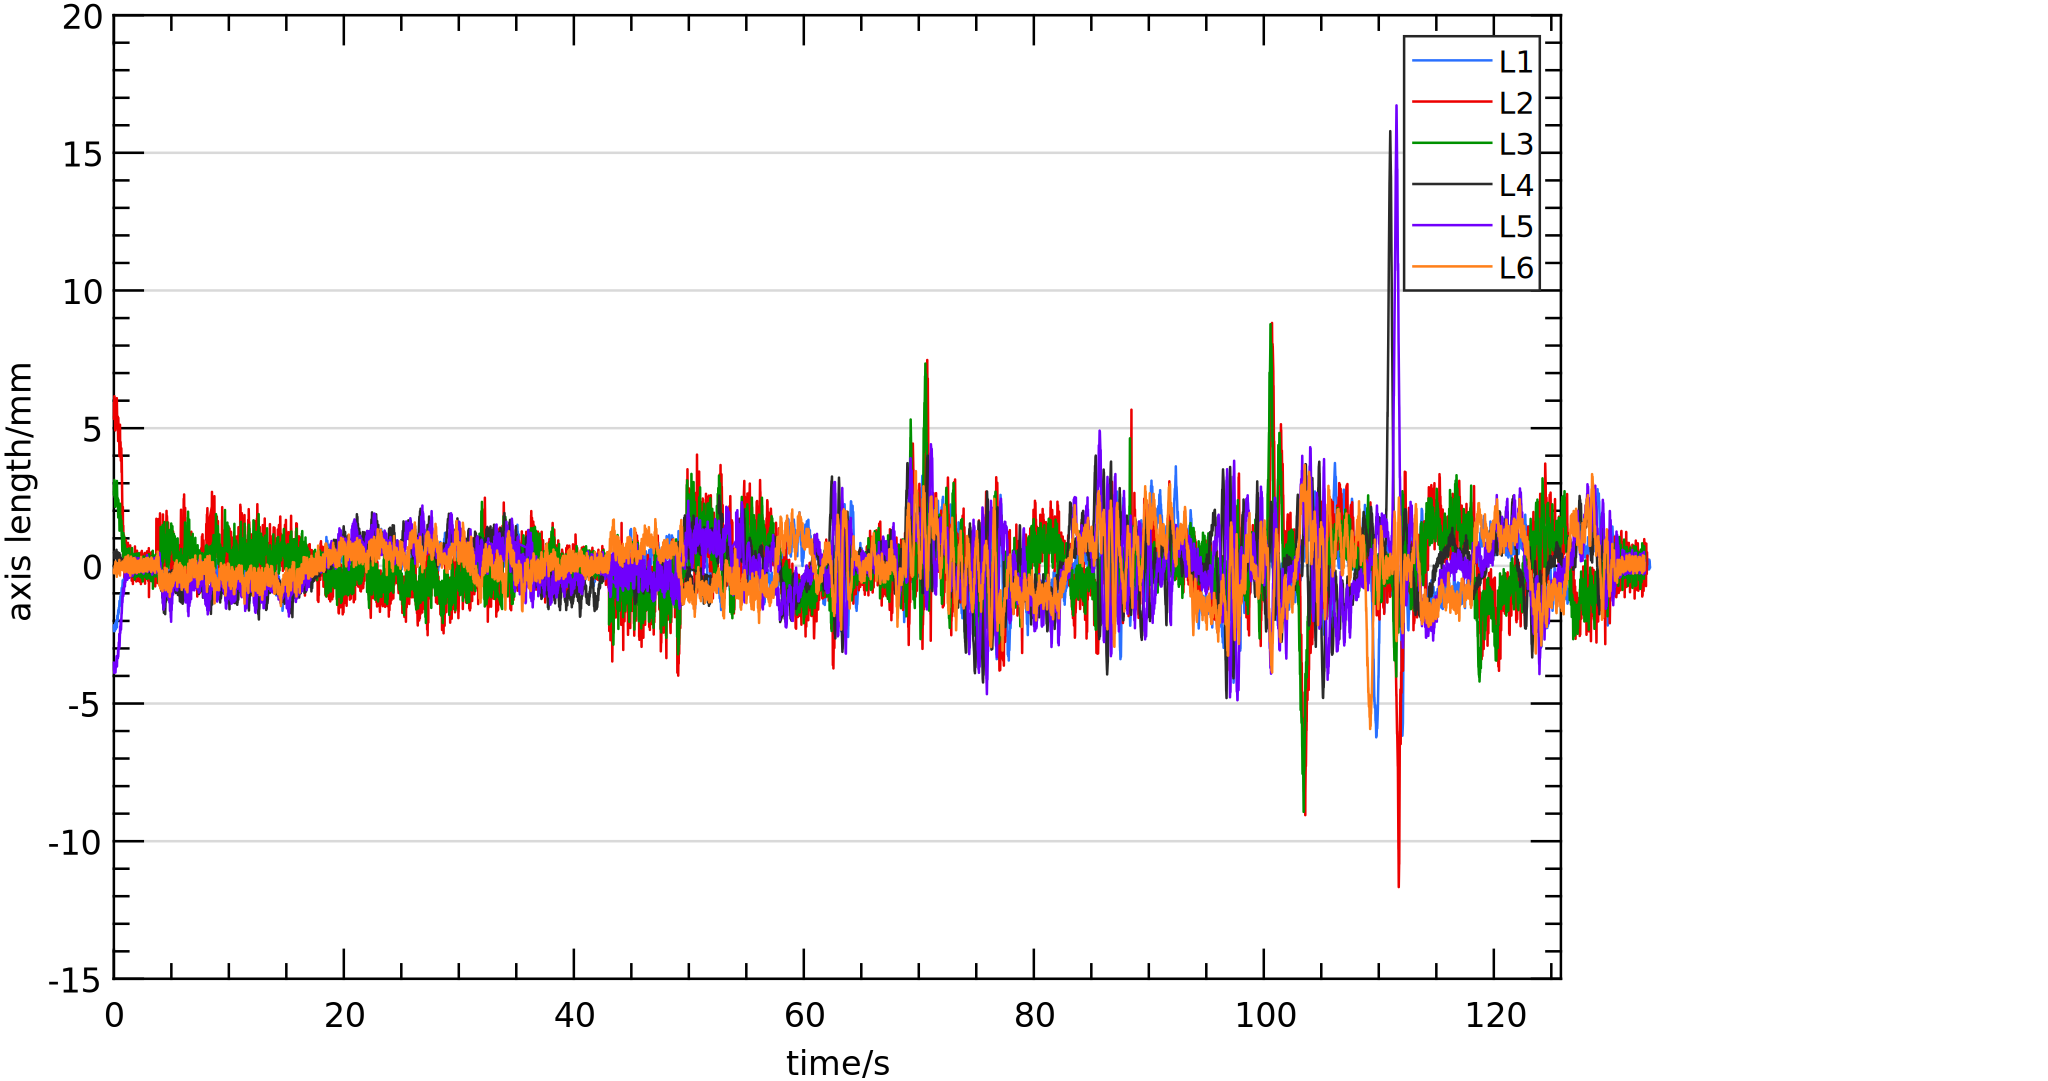
\includegraphics[width=0.6\textwidth]{imgs/Experiment/C-AH-FL_1_axis_diff_length.png}
    \caption{凸优化-自适应滑膜控制器在输入高振幅、低频率情况下的轴长跟踪误差}
    \label{fig:C-AH-FL_1_axis_diff_length}
\end{figure}

\begin{figure}[H]
    \centering
    \includegraphics[width=0.6\textwidth]{imgs/Experiment/C-AH-FL_1_c_movement.png}
    \caption{凸优化-自适应滑膜控制器在输入高振幅、低频率情况下,正解得到的C平台位置移动情况}
    \label{fig:C-AH-FL_1_c_movement}
\end{figure}

在图\ref{fig:C-AH-FL_1_axis_diff_length}中棕色虚线左半边是输入主要为x,y,z三方向对应的幅值变化,右半边的输入则主要是角度变化。可以发现,左半边的抑振效果明显好于右半边,这是因为机构的特性导致的。当机构发生角度偏转时,类似于倒立摆,顶部的C平台的运动会被放大。粗略的计算可以得到,输入角度每变化1度,相当于C平台移动20mm,因此一旦角度变化速度快,凸优化规划器就会限制输出速度,从而导致跟踪误差增大。因此,下面分析输入主要以位置变化的情形为主,角度变化阶段不做考虑。

对每根轴而言,从图\ref{fig:C-AH-FL_1_axis_diff_length}可以看出,其在位置变化阶段基本可以将跟踪误差控制在$\pm 1 \mathrm{mm}$之间,而其变动范围基本为$50 \mathrm{mm}$,即相对的控制精度可以达到$2\%$。从图\ref{fig:C-AH-FL_1_c_movement}可以看出,位置变化情形下,通过本文提出的凸优化-自适应滑膜控制器,可以将C平台每个轴的位置误差控制在$\left[ -5\mathrm{mm},3\mathrm{mm} \right] $左右(其中x轴曲线存在一个$-5\mathrm{mm}$的静偏差,是因为控制开始时的初始位置不同导致的)。

相比输入的幅值条件:x轴$[-40\mathrm{mm}, 50\mathrm{mm}]$,y轴$\left[ -35\mathrm{mm},45\mathrm{mm} \right] $的情况,其幅值范围被抑制到接近$10\%$。对比前文提出的控制要求,这里得到的控制结果优于控制指标。

% todo rms 指标
% \textbf{是否需要计算RMS指标}

对低振幅,高频率的情形,其结果为图\ref{fig:C-AL-FM_1_input}-\ref{fig:C-AL-FM_1_c_movement}:

\begin{figure}[H]
    \centering
    \subfloat[输入扰动x,y,z三方向振幅]{
    \begin{minipage}[t]{0.4\linewidth}
    \centering
    \includegraphics[width=0.9\textwidth]{imgs/Experiment/C-AL-FM_1_position_B_error.png}
    % \caption{}
    \end{minipage}%
    }%
    \hspace{0.5pt}
    \subfloat[输入扰动RPY角振幅]{
    \begin{minipage}[t]{0.4\linewidth}
    \centering
    \includegraphics[width=0.9\textwidth]{imgs/Experiment/C-AL-FM_1_rpy_B.png}
    % \caption{}
    \end{minipage}%
    }%
    \centering
    \caption[]{凸优化-自适应滑膜控制器对应的输入扰动振幅}
    \label{fig:C-AL-FM_1_input}
\end{figure}

\begin{figure}[H]
    \centering
    \subfloat[6轴实际轴长]{
    \begin{minipage}[t]{0.4\linewidth}
    \centering
    \includegraphics[width=0.9\textwidth]{imgs/Experiment/C-AL-FM_1_axis_actual_length.png}
    % \caption{}
    \end{minipage}%
    }%
    \hspace{0.5pt}
    \subfloat[6轴期望轴长]{
    \begin{minipage}[t]{0.4\linewidth}
    \centering
    \includegraphics[width=0.9\textwidth]{imgs/Experiment/C-AL-FM_1_axis_ideal_length.png}
    % \caption{}
    \end{minipage}%
    }%
    \centering
    \caption[]{凸优化-自适应滑膜控制器在输入低振幅、高频率情况下的轴长响应图}
    \label{fig:C-AL-FM_1_axis}
\end{figure}

\begin{figure}[H]
    \centering
    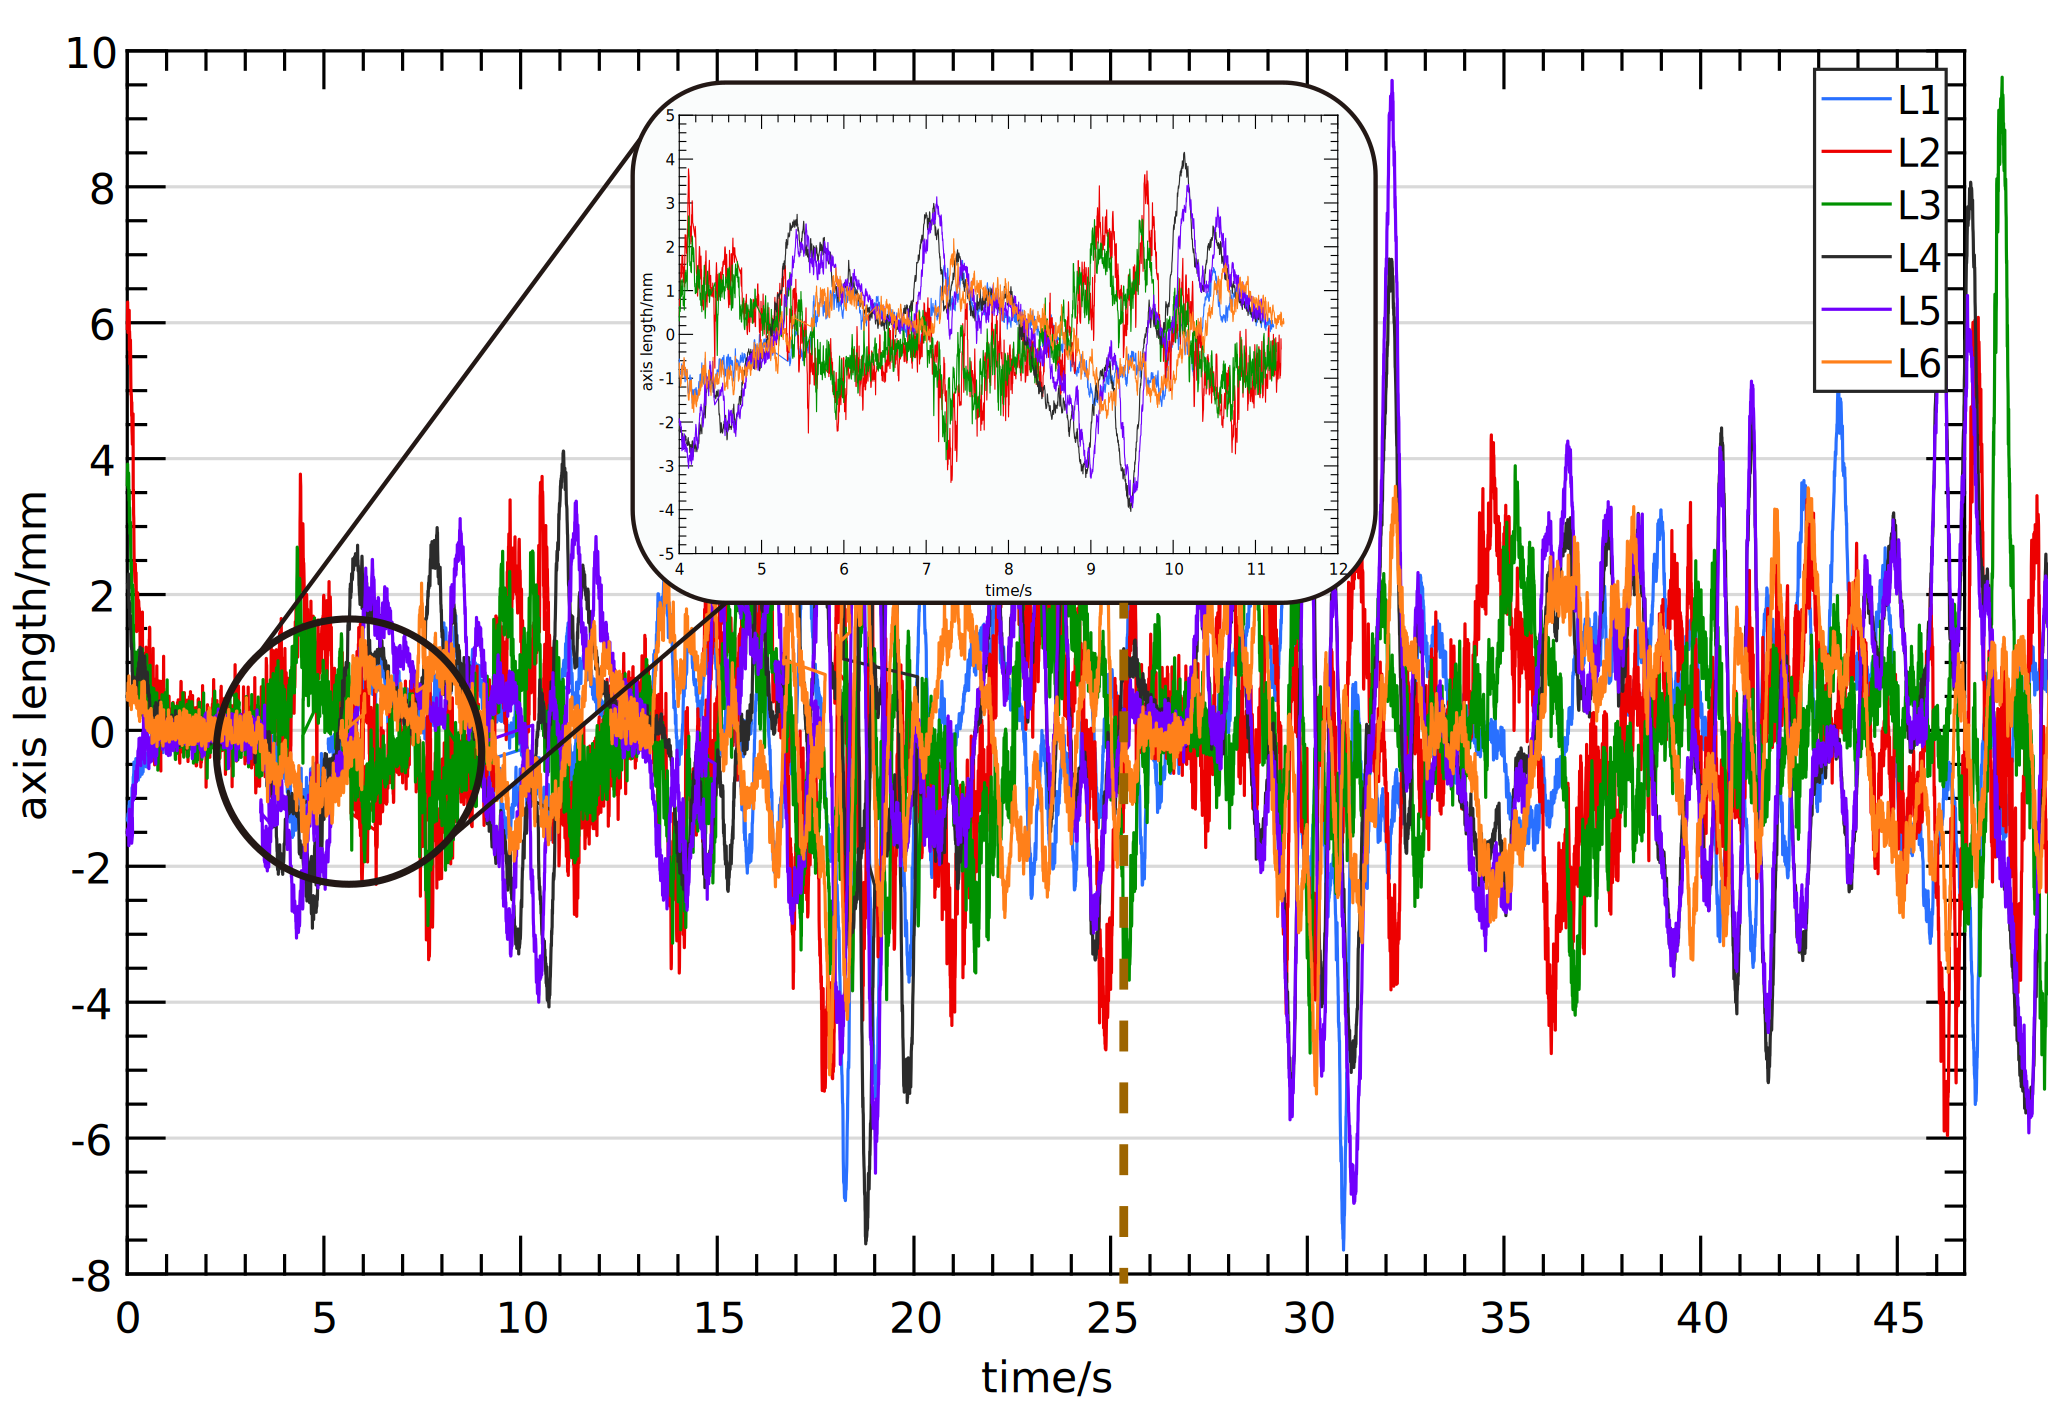
\includegraphics[width=0.6\textwidth]{imgs/Experiment/C-AL-FM_1_axis_diff_length.png}
    \caption{凸优化-自适应滑膜控制器在输入低振幅、高频率情况下的轴长跟踪误差}
    \label{fig:C-AL-FM_1_axis_diff_length}
\end{figure}

\begin{figure}[H]
    \centering
    \includegraphics[width=0.6\textwidth]{imgs/Experiment/C-AL-FM_1_c_movement.png}
    \caption{凸优化-自适应滑膜控制器在输入低振幅、高频率情况下,正解得到的C平台位置移动情况}
    \label{fig:C-AL-FM_1_c_movement}
\end{figure}

对比前面高振幅、低频率的情形,此时尽管输入的振幅减小为之前的一半左右,但其变化频率明显增大。在15s前,对应的轴的跟踪精度下降,每根轴误差被放大到
$\left[ -3\mathrm{mm},4\mathrm{mm} \right] $,而C平台的控制精度则降低到$\left[ -5\mathrm{mm},5\mathrm{mm} \right] $(x轴)。在15s后,y轴振动速度更快,此时轴的跟踪精度下降到$\left[ -6\mathrm{mm},6\mathrm{mm} \right] $,C平台的精度下降到$\left[ -10\mathrm{mm},10\mathrm{mm} \right] $,且可以发现,C平台在y轴方向振动很厉害。这表明控制器这样的高频下跟踪精度下降很快,同时凸优化规划器在这里也起了一定的作用,类似一个低通滤波器将轨迹平滑了。

对比PID控制器在高振幅、低频率下的控制情况,结果如图所示:

\begin{figure}[H]
    \centering
    \subfloat[输入扰动x,y,z三方向振幅]{
    \begin{minipage}[t]{0.4\linewidth}
    \centering
    \includegraphics[width=0.9\textwidth]{imgs/Experiment/P-AH-FL_1_position_B_error.png}
    % \caption{}
    \end{minipage}%
    }%
    \hspace{0.5pt}
    \subfloat[输入扰动RPY角振幅]{
    \begin{minipage}[t]{0.4\linewidth}
    \centering
    \includegraphics[width=0.9\textwidth]{imgs/Experiment/P-AH-FL_1_rpy_B.png}
    % \caption{}
    \end{minipage}%
    }%
    \centering
    \caption[]{PID控制器对应的输入扰动振幅}
    \label{fig:P-AH-FL_1_input}
\end{figure}

\begin{figure}[H]
    \centering
    \subfloat[6轴实际轴长]{
    \begin{minipage}[t]{0.4\linewidth}
    \centering
    \includegraphics[width=0.9\textwidth]{imgs/Experiment/P-AH-FL_1_axis_actual_length.png}
    % \caption{}
    \end{minipage}%
    }%
    \hspace{0.5pt}
    \subfloat[6轴期望轴长]{
    \begin{minipage}[t]{0.4\linewidth}
    \centering
    \includegraphics[width=0.9\textwidth]{imgs/Experiment/P-AH-FL_1_axis_ideal_length.png}
    % \caption{}
    \end{minipage}%
    }%
    \centering
    \caption[]{PID控制器在输入低振幅、高频率情况下的轴长响应图}
    \label{fig:P-AH-FL_1_axis}
\end{figure}

\begin{figure}[H]
    \centering
    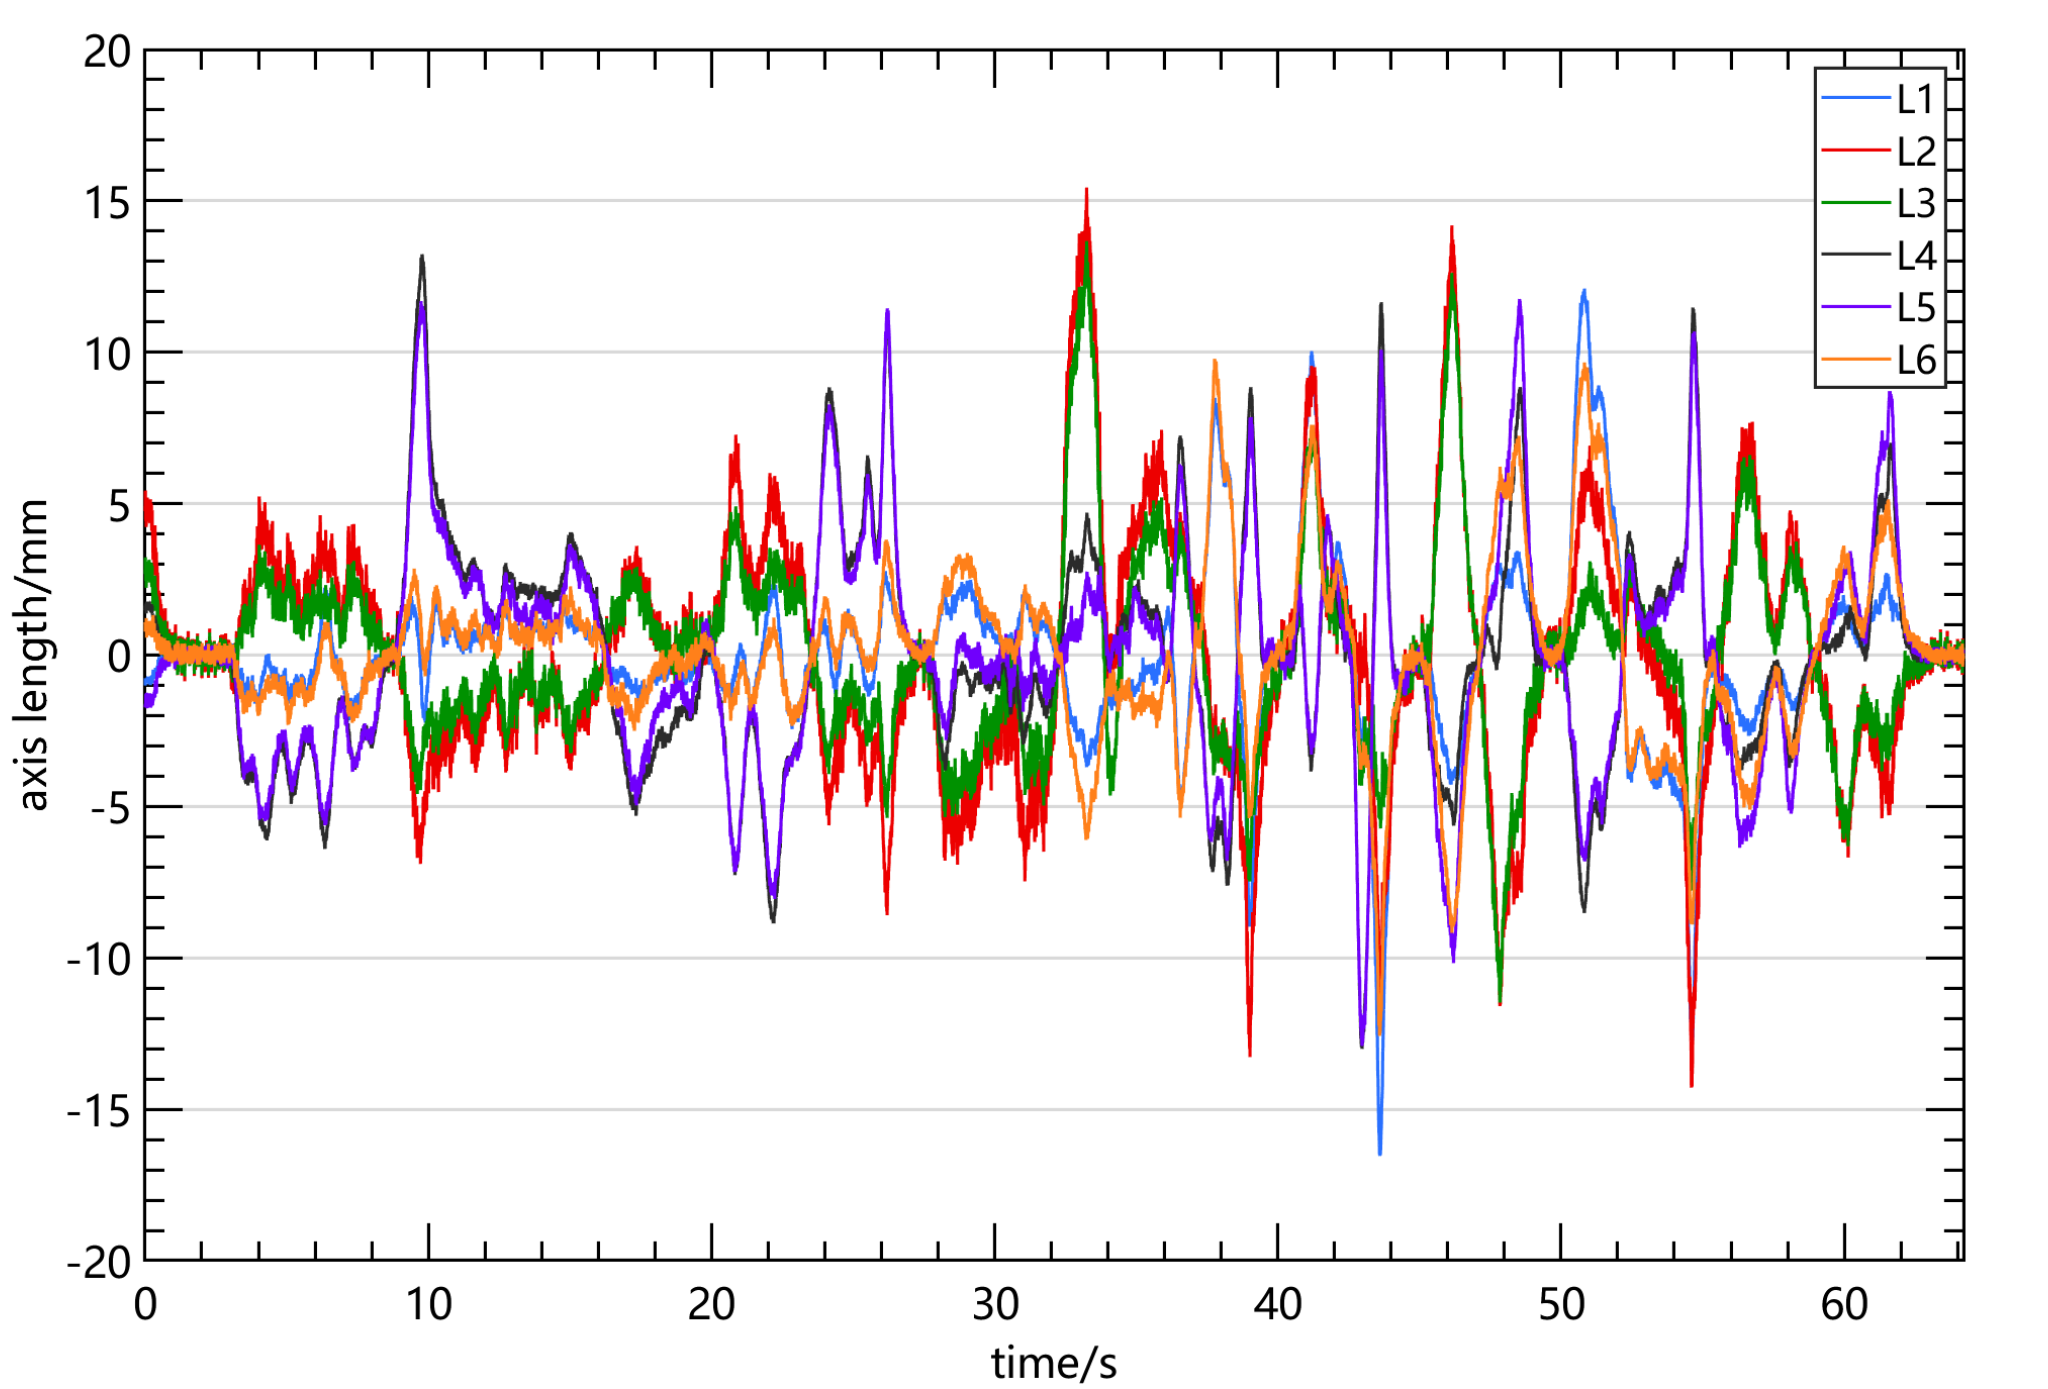
\includegraphics[width=0.6\textwidth]{imgs/Experiment/P-AH-FL_1_axis_diff_length.png}
    \caption{PID控制器在输入低振幅、高频率情况下的轴长跟踪误差}
    \label{fig:P-AH-FL_1_axis_diff_length}
\end{figure}

\begin{figure}[H]
    \centering
    \includegraphics[width=0.6\textwidth]{imgs/Experiment/P-AH-FL_1_c_movement.png}
    \caption{PID控制器在输入低振幅、高频率情况下,正解得到的C平台位置移动情况}
    \label{fig:P-AH-FL_1_c_movement}
\end{figure}

对比PID控制器和本文提出的滑膜控制器结果,可以发现,其轴的跟踪精度在$\left[ -6\mathrm{mm},10\mathrm{mm} \right] $
左右,对应的C平台位置精度为$x:\left[ -6\mathrm{mm},6\mathrm{mm} \right] ,y:\left[ -10\mathrm{mm},10\mathrm{mm} \right] $,其精度差于本文的控制器。

如果直接将逆解轴长作为控制量进行控制,其结果为:

\begin{figure}[H]
    \centering
    \subfloat[输入扰动x,y,z三方向振幅]{
    \begin{minipage}[t]{0.4\linewidth}
    \centering
    \includegraphics[width=0.9\textwidth]{imgs/Experiment/N-AH-FL_1_position_B_error.png}
    % \caption{}
    \end{minipage}%
    }%
    \hspace{0.5pt}
    \subfloat[输入扰动RPY角振幅]{
    \begin{minipage}[t]{0.4\linewidth}
    \centering
    \includegraphics[width=0.9\textwidth]{imgs/Experiment/N-AH-FL_1_rpy_B.png}
    % \caption{}
    \end{minipage}%
    }%
    \centering
    \caption[]{无控制器时的输入扰动振幅}
    \label{fig:N-AH-FL_1_input}
\end{figure}

\begin{figure}[H]
    \centering
    \subfloat[6轴实际轴长]{
    \begin{minipage}[t]{0.4\linewidth}
    \centering
    \includegraphics[width=0.9\textwidth]{imgs/Experiment/N-AH-FL_1_axis_actual_length.png}
    % \caption{}
    \end{minipage}%
    }%
    \hspace{0.5pt}
    \subfloat[6轴期望轴长]{
    \begin{minipage}[t]{0.4\linewidth}
    \centering
    \includegraphics[width=0.9\textwidth]{imgs/Experiment/N-AH-FL_1_axis_ideal_length.png}
    % \caption{}
    \end{minipage}%
    }%
    \centering
    \caption[]{无控制器时,输入低振幅、高频率情况下的轴长响应图}
    \label{fig:N-AH-FL_1_axis}
\end{figure}

\begin{figure}[H]
    \centering
    \includegraphics[width=0.6\textwidth]{imgs/Experiment/N-AH-FL_1_axis_diff_length.png}
    \caption{无控制器时,输入低振幅、高频率情况下的轴长跟踪误差}
    \label{fig:N-AH-FL_1_axis_diff_length}
\end{figure}

\begin{figure}[H]
    \centering
    \includegraphics[width=0.6\textwidth]{imgs/Experiment/N-AH-FL_1_c_movement.png}
    \caption{无控制器时,输入低振幅、高频率情况下,正解得到的C平台位置移动情况}
    \label{fig:N-AH-FL_1_c_movement}
\end{figure}

可以发现,直接将轴长作为控制量进行控制,最终轴的跟踪精度在$\left[ -6\mathrm{mm},10\mathrm{mm} \right] $左右,对应的C平台位置精度为$x:\left[ -15\mathrm{mm},15\mathrm{mm} \right] ,y:\left[ -5\mathrm{mm},10\mathrm{mm} \right] $,其精度比PID差一点。这是因为如果直接将轴长进行反馈,轴的运动会产生反作用力,改变B的位姿,从而使C的位姿发生变化。因为控制周期不能无限小,因此这样做会不断产生误差,甚至在一定频率下,由支链的反作用力作为驱动发生激振。

% todo: 列出结果的表格,作为结束

实验结果表明,本文提出的控制器对悬浮的Stewart机构在外力扰动下的振动抑制有一定的作用。在频率较低的情况下,可以将振幅抑制为$10\%$左右;而对频率高的情况下,控制器做了安全措施来限制输出速度,保证机构安全的同时也使得跟踪误差增大。实验结果也验证了仿真分析得到的控制算法特点:

\begin{enumerate}
    \item 控制器是基于无模型的控制
    \item 控制器对噪声鲁棒,抗干扰能力强
    \item 控制器输出受限,保证仪器安全
    \item 控制器收敛速度快
\end{enumerate}
\FloatBarrier


\section{结论}

本文针对FAST机构对应的悬浮的Stewart结构,由于其复杂的动力学特征和难以辨识的参数的特征,提出了一种无模型的自适应滑膜控制器,可以快速、鲁棒地完成轨迹跟踪的任务。在此基础上,为了保证机构稳定运行,设计了凸优化的轨迹规划器来保证运动处于机构安全范围内。最终,在搭建的FAST缩尺机构上完成了抑振实验,其控制精度满足缩尺实验的要求。



% 生成参考文献
\bibliography{ref}

\end{document}